\section{Text Representation in Legal Judgments}\label{sec:text_representation}

% Resumo do obj

The experiments and results presented in this section are related to text representation. First, there is the clarification of the experiments' purpose, and how they answer the research question. Then, it presents the details on the datasets, the pipelines, the results, and the discussion.\footnote{The code for training and evaluating embeddings is available at \url{https://github.com/thiagordp/embeddings_in_law_paper}.}




\subsection{Experiment's Purpose}

% \begin{itemize}[noitemsep]
%     \item Cronologia
%     \item Falta de representação para o juridico  em português.
%     \item Avaliar se a especificade e tamanho do corpus ajudam em alguma coisa.
%     \item Avaliar como aprendizado profundo se sai na classificação das sentenças.
%     \item Como ajuda responder a segunda pergunta?
% \end{itemize}

The experiments' purpose is to answer the first part of the research question, i.e., whether the size and specificity of the corpus used for word embedding training impact the performance in a classification task. 
Thus, the experiments from this section focus on the aspects of training and testing word embeddings representations. The first step is the datasets construction, where we collected two types of data: unlabeled corpora for training embeddings and labeled dataset for classification. Significant part of those datasets were not available for use in any dataset platform, such as Kaggle, and had to be collected and prepared, producing a considerable amount work. Also, a legal expert manually labeled each of the legal judgments from the second dataset.


To answer the research question the unlabeled corpora is used to train several word embeddings representations, while varying corpora sizes and degrees of specificity (also called \textit{context}). To do so, the corpora is divided in three, according to specificity: corpus related to all subjects, corpus related to all legal subjects and corpus related to air transport services and the legal domain. 
After that, each of those three corpora is divided is several subsets to form other corpora with distinct  corpus size. 
For each of the smaller corpora, we trained word embeddings models using GloVe technique, as we detailed later. Finally, we apply each resulting  embeddings model as representation in the classification task for evaluation.


The tools for the experiments in this section embraced the collection and the preprocessing of the data, as well as the embeddings training and the text classification. To collect most of the unlabeled corpora, we used Selenium~\cite{Salunke2014}, while the text prepreprocessing involved the \gls{NLTK}~\cite{Loper02}. In the classification task, we applied the Keras Framework optimized to run on \gls{GPU}.   As programming language, we adopted Python  to build the experimental setup.


Finally, another aim of these experiments is to build and make available pre-trained representations which can be used by other researchers in their own \gls{TM} experiments with legal documents in Portuguese.



\subsection{Dataset} \label{sec:embedding_dataset}

% Porque só três tribunais? 


% Informar a estrutura da sentença:
% Porque faz sentido usar o texto final ao invés da petição inicial?


The first dataset is a collection of legal documents from the courts web portals, which  enable us to evaluate the specificity influence of these legal corpora. We divided the dataset into two contexts: related to general legal texts and related to air transport services text.

% Warning!! Copy/Paste
Another dataset is a collection of texts from other general topics (not related to legal domains) that are already compiled and freely available. Having the corpora for legal and miscellaneous contexts, we applied some processing steps to remove noise from texts. To evaluate the influence of corpus size in embeddings training, we divided these three corpora into smaller pieces based on word count.

% Warning!! Copy/Paste 
To train the embeddings it is required large text corpora to be able to get good embeddings. However, in the Brazilian Portuguese language, we could not find any dataset available on the Internet containing enough legal text corpora for our purposes. Thus, we had to build our legal corpora.

% Warning!! Copy/Paste 
Our main sources of legal text are Brazilian courts platforms. We collected judgments from the webpages of \gls{STF}, \gls{STJ} and \gls{TJ-SC}~\cite{STF2020, STJ2020, TJSC2020}. 
We also collected judgments from the JusBrasil portal containing processes related only to failures on air transport service from all \gls{TJ} from Brazil~\cite{Jusbrasil2020}. We choose those courts based on the hierarchy of the Brazilian Judiciary presented in Figure~\ref{fig:courts}.

\begin{figure}[htb]
    \centering
    \caption{Brazilian Judiciary hierarchical structure}
    \label{fig:courts}
    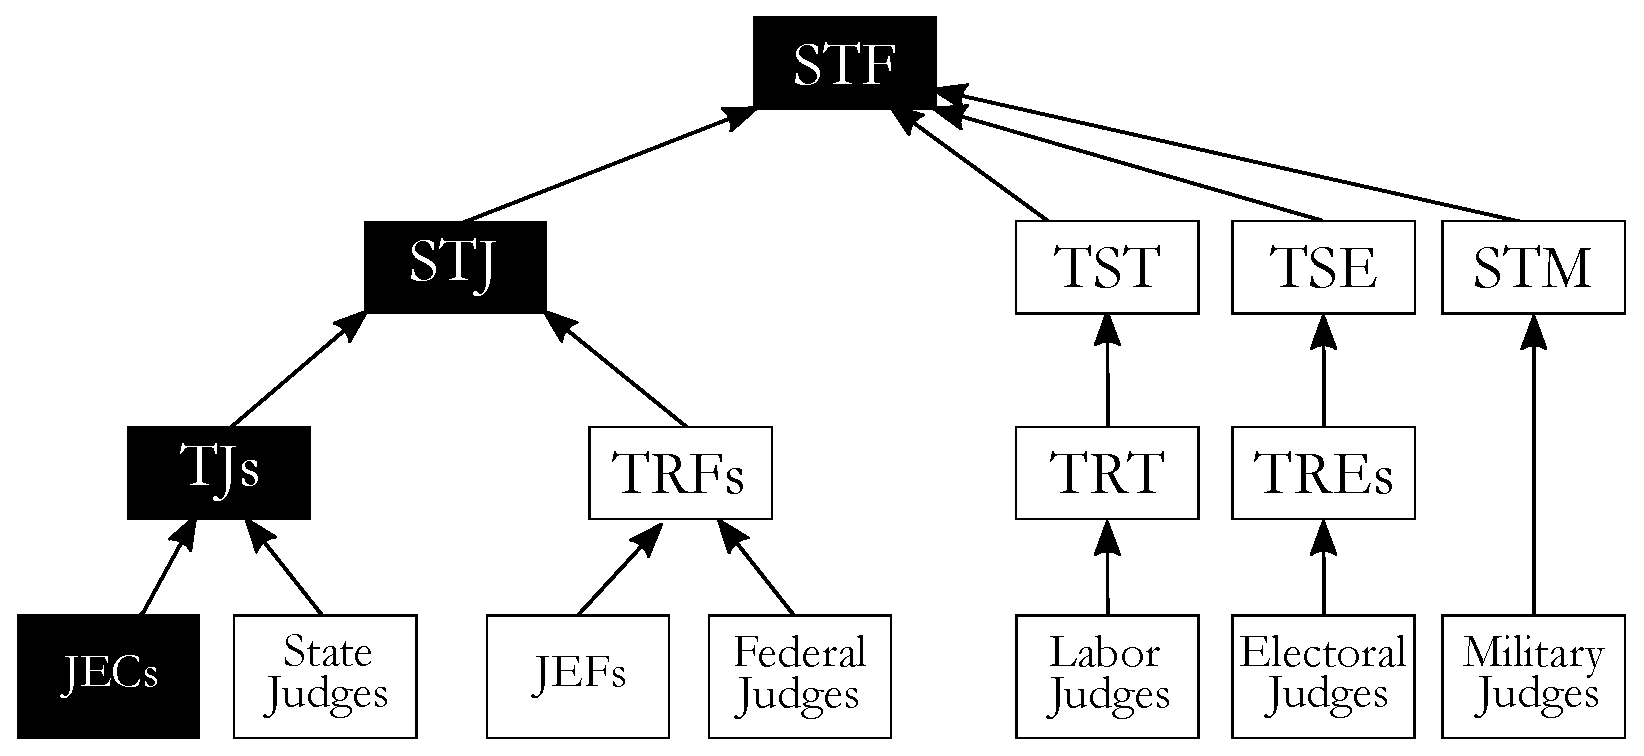
\includegraphics[width=0.8\textwidth]{images/chapters/fig1_courts.eps}
\end{figure}

Considering that the documents used in the task classification came from the \gls{JEC} at \gls{UFSC}, we follow the structure starting from \gls{JEC} at the lower level until the \gls{STF} at the top. As the higher courts judge the appeals of lower courts, the legal judgments' subjects from the higher courts may have a degree of similarity to the judgments from \gls{JEC}.

% Warning!! Copy/Paste 
Table~\ref{tab:count_process} shows the number of processes acquired and word count for each court.

\begin{table}[htb]
\caption{Acquired legal judgments from courts for embeddings training}
\label{tab:count_process}
\footnotesize
\centering
\begin{tabular}{@{}crrrr@{}}
\toprule
\textbf{Source}      & \multicolumn{1}{c}{\textbf{\begin{tabular}[c]{@{}c@{}}Collegial \\ Judgments\end{tabular}}}   & \multicolumn{1}{c}{\textbf{\begin{tabular}[c]{@{}c@{}}Individual \\ Judgments\end{tabular}}} & \multicolumn{1}{c}{\textbf{Subtotal}} &\multicolumn{1}{c}{\textbf{\begin{tabular}[c]{@{}c@{}}Word \\ Count\end{tabular}}} \\ \midrule
STF                  & 64,779              & 118,910              & 183,689     & 294,937,185  \\
STJ                  & 101,141              & 0                    & 101,141      & 312,687,450 \\
TJ-SC                & 989,964              & 662,535              & 1,652,499   & 3,060,212,814  \\
TJs (JusBrasil)           & 34,239               & 0                    & 34,239        & 78,138,337\\ \midrule
\multicolumn{1}{l}{} & \multicolumn{1}{l}{} & \textbf{TOTAL}       & 1,971,568     &  3,745,975,786\\ \bottomrule
\end{tabular}

%\fonte{\textcite{DalPont2020}.}
\end{table}

% Warning!! Copy/Paste 
After downloading all the legal judgments, most of them in \gls{PDF} and \gls{RTF}, we extracted raw texts from these files. We did not apply \gls{OCR} in scanned PDF documents, due to time limits to finish the experiments, so only digital \gls{PDF}  and \gls{RTF} files were accounted in Table~\ref{tab:count_process}. 

% Warning!! Copy/Paste 
With the extracted texts, we applied some preprocessing steps, as discussed further in this section. 

% Warning!! Copy/Paste 
Then we built the legal text corpora containing all the judgments related to all law subjects, which we call \emph{general} legal context corpora in this work. Using this base, we created another text corpora whose legal judgments are related only to air transport and consumer law, and we call it \emph{air transport} context corpora.

% Warning!! Copy/Paste 
To be able to compare how good embeddings trained with legal texts perform against those created with all kinds of texts, we also created other corpora from a variety of sources. Thus, we searched for free available textual datasets. In this work, we call these texts as \emph{global} context corpora. Table~\ref{tab:global_corpora} shows all the global text datasets used. Then we apply some preprocessing steps, as will be described further in this section.

\begin{table}[htb]
\caption{Global context corpora for embeddings training}
\label{tab:global_corpora}
\centering
\footnotesize
\begin{tabular}{@{}crrc@{}}
\toprule
\textbf{Dataset}                   & \textbf{Documents} & \textbf{Word Count} & \textbf{Source} \\ \midrule
Wikipedia in Portuguese            & 1,014,713          & 303,622,360         & \textcite{Wikipedia2019}                \\
Brazilian Literature Books         & 169                & 37,848,783          & \textcite{Tatman2017}                 \\
Old Newspapers                     & 617,627            & 26,441,581          &         \textcite{Tan2020}     \\
Folha de São Paulo News            & 165,641            & 74,594,367          &                     \textcite{Marlessonn2019}             \\
HC News Corpus                     & 494,128            & 27,170,063          &        \textcite{Christensen2016}         \\
Blogspot Posts                     & 2,181,073          & 696,657,915         &          \textcite{Santos2018}       \\
Wikihow Instructions               & 786,283            & 22,471,312          &        \textcite{Chocron2018}         \\ \midrule
\multicolumn{1}{r}{\textbf{TOTAL}} & 5,259,634          & 1,188,806,381       & \textbf{}       \\ \bottomrule
\end{tabular}

% \fonte{\textcite{DalPont2020}.}
\end{table}

The dataset for evaluation in the classification task is composed of almost one thousand legal judgments from the \gls{JEC} at \gls{UFSC}, issued between January 2014 to November 2019, and collected manually by a legal expert on site. The specific subject debated is failures in air transport services, such as flight delay, flight cancellation, baggage loss. Then the consumer injured claims compensation for immaterial damage, which is a monetary value fixed by the judge. 

% Não precisa
% The legal judgments refer only to situations in which consumers had problems with airlines. To solve them, the Code of Consumer Protection provides basic consumer's rights, such as effective compensation for material and immaterial damages, and ways to facilitate consumer's defense and ensure their rights. One of these is through Special Courts since it offers an unbureaucratic way out to solve their problems~\cite{Brazil1990}. 

% Não precisa
% Immaterial damage is an injury to personality rights, such as honor, dignity, intimacy, image, name~\cite{Goncalves2011}. Regarding the failures in air transport service, for example, flight delay, flight cancellation or baggage loss, the courts have been decided that they can generate immaterial damage and consumer compensation~\cite{Benjamim2015}. 

Compensation for immaterial damage is usually monetary. It is not possible to evaluate the painful sensation experienced by the injured person. As a mean of mitigating the consequences, money can play a satisfactory role~\cite{Diniz2020}. There are some circumstances considered by the judge when fixing the value, such as the person’s age, health status, person’s gender, place and time of injury. Anyway, these variables are weighted by the judge in a free assessment, according to his/her interpretation of each situation~\cite{Sadiku2020}.

A legal judgment is an unstructured textual document and refers to the final decision of a lawsuit in first degree. Generally, it consists of three elements~\cite{Brazil2015}:

\begin{itemize}[noitemsep]
    \item \emph{Report} (summary of what happened according to the parties allegations and evidences);
    \item \emph{Reasoning} (reasons that formed the judge's conviction);
    \item \emph{Result} (value fixed by the judge for immaterial damage compensation). 
\end{itemize}

There are four possible labels for the legal judgments:

\begin{itemize}[noitemsep]
    \item \textit{Well-founded:} The consumer wins the lawsuit, 26\% of the dataset.
    \item \textit{Not founded:} The consumer loses the lawsuit, 10\% of the dataset.
    \item \textit{Partly founded:} The consumer wins part of the lawsuit (for example, when he/she plead a greater compensation than the assigned value by the judge), 62\% of the dataset.
    \item \textit{Dismissed without prejudice:} The consumer makes a procedural error (for example, when he/she indicates as a defendant the wrong airline company). So the consumer can file a new lawsuit, 2\% of the dataset.
\end{itemize}

In the experiments from this section, to evaluate the representations using text classification, we removed the judgments' result part. Thus, to make predictions the \gls{ML} techniques will have the summary of the facts and the legal reasoning, that is the same data available at the early stages  of a real case.
Applying this approach, we could execute experiments while overcoming the difficulties of acquiring data from the early stages of lawsuits.

\subsection{Pipeline}\label{sec:pipeline_representation}

 
This section describes the pipelines and experimental setup for the experiments of embeddings training and evaluation.
 
The first part of the experiments consisted on training the word embeddings models based on  unlabeled corpora. 
%In such experiments, we used a set of programming tools such as Selenium \cite{Salunke2014}, to collect and extract the unlabeled corpora. Another set of tools was used to preprocess the text and train the embeddings, that is, \gls{NLTK} and  Gensim. At the end of this first part we had the trained word embeddings.
The second part of the experiments involved the evaluation of the embeddings in a text classification task of the legal judgments from \gls{JEC}, using the trained embeddings to represent the text.
 
Figure~\ref{fig:pipeline_embeddings} shows the pipeline used in the experiments from this section.
%pipeline for embeddings training and evaluation

\begin{figure}[htb]
    \centering
    \caption{Pipeline for embeddings training and evaluation}
    \label{fig:pipeline_embeddings}
    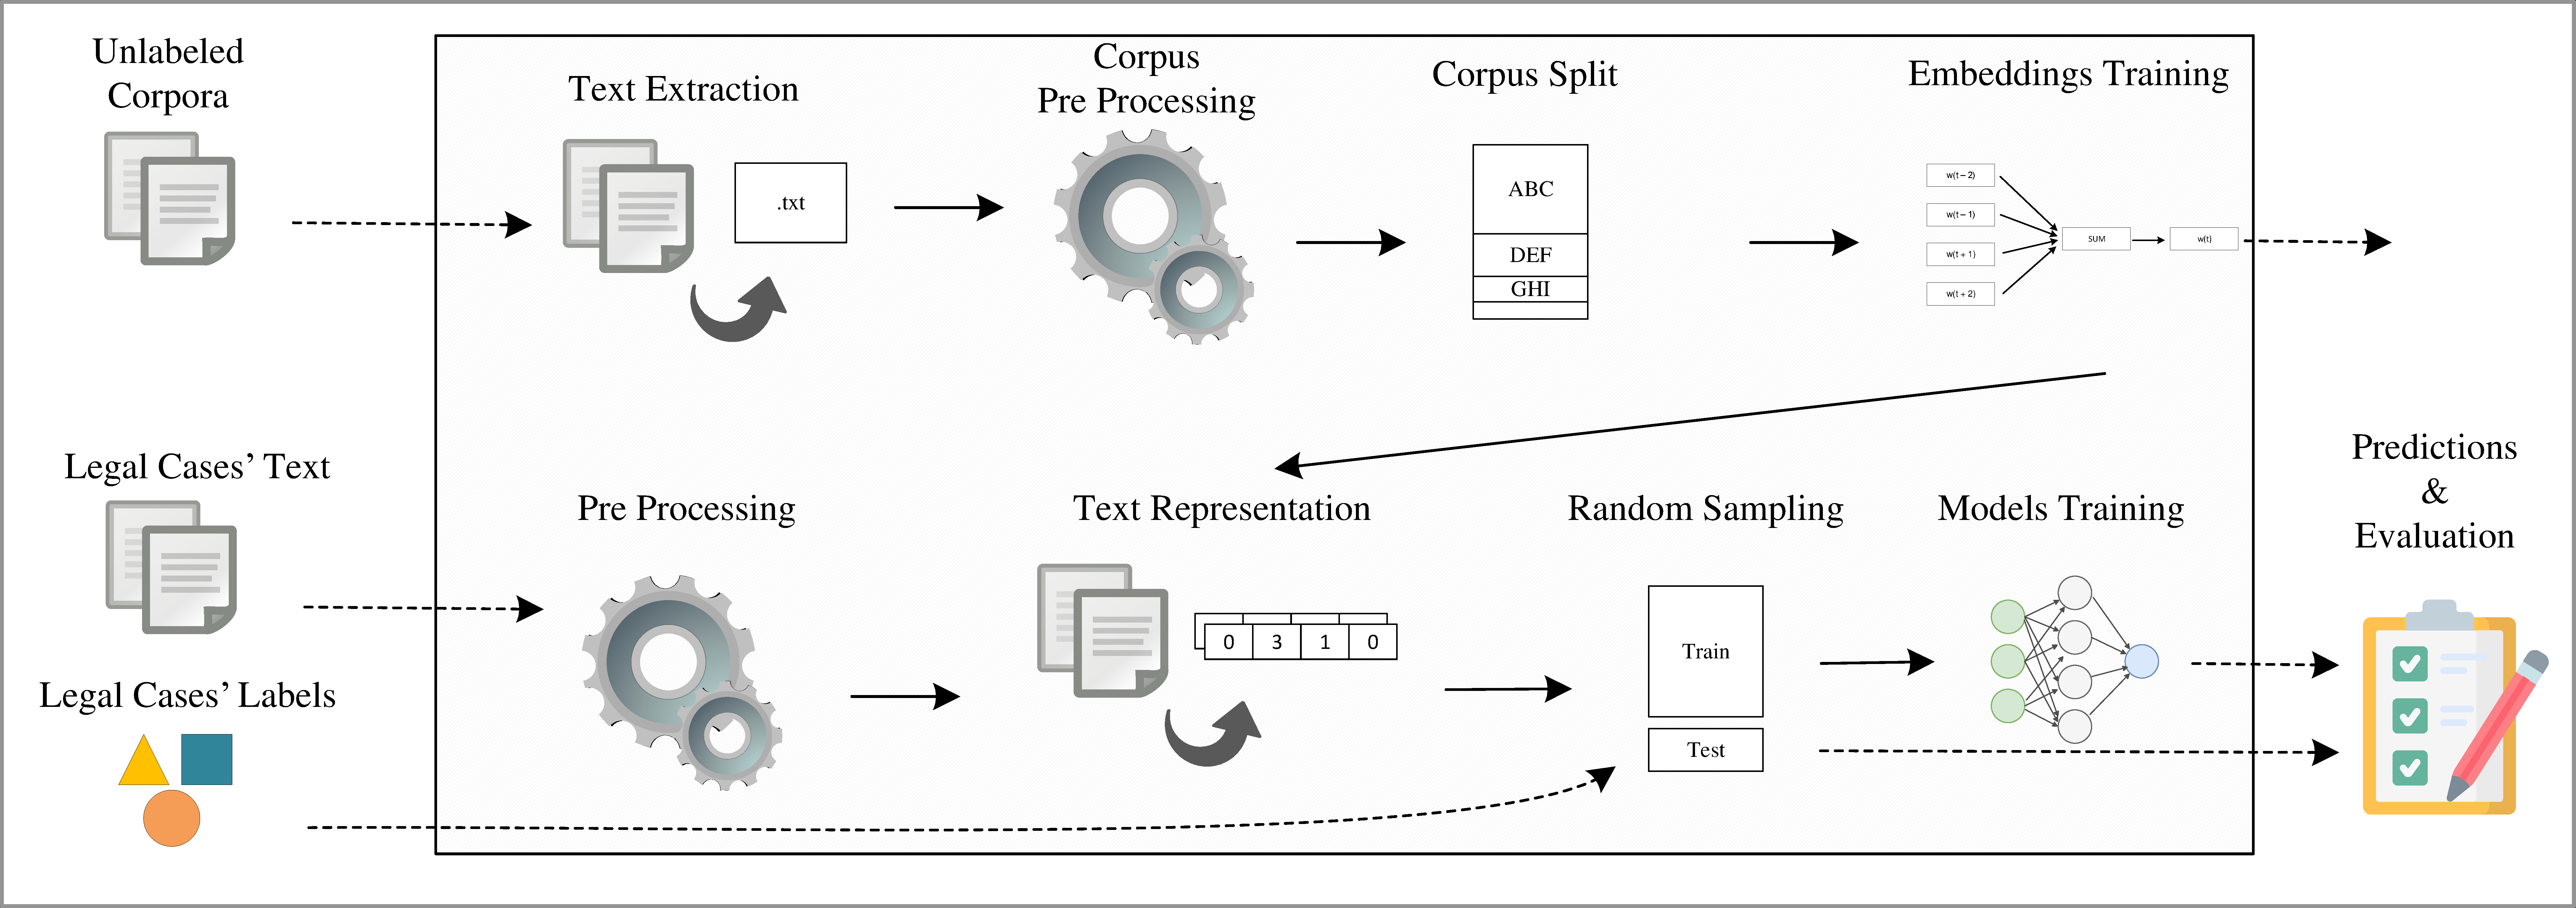
\includegraphics[width=\textwidth]{images/chapters/cap4_proposed_pipeline_embeddings.pdf}
\end{figure}

% Warning!! Copy/Paste

The pipeline from Figure~\ref{fig:pipeline_embeddings} receives three types of input: the unlabeled corpora, the legal judgments' text and the labels. In terms of output, there are three types: the trained embeddings, the classification models and the test set.

The first step in the pipeline is the text extraction, where the original files in \gls{PDF} and \gls{RTF} are converted to raw text format.
%
After text extraction, we applied some preprocessing steps, required before training the embeddings, as follows: the conversion to lower case and the removal of punctuation marks, special characters and symbol characters. We did not removed stopwords or apply stemmization or lemmatization, following the literature~\cite{Mikolov2013, Pennington2014}.


In the next step, there is the corpora split where the texts are divided in subsets. The three complete corpora comprised 3.7 billion, 100 million  and 1.19 billion words for \emph{general}, \emph{air transport} and \emph{global} corpora, respectively. The possible sizes of the subsets, considering word count are: 1,000; 10,000; 50,000; 100,000; 200,000; 500,000; 1,000,000; 5,000,000; 10,000,000; 25,000,000; 100,000,000; 500,000,000; 750,000,000 and 1,000,000,000.

We choose these corpora sizes to be able to compare the variation on performance metrics while increasing corpora size. For the air transport context, we could not embrace all these sizes due to limited corpora available. The largest subset for this context had 100 million words. 

Finally, each of the subsets (smaller corpora) was used to train distinct word embeddings representation.

As word embeddings technique, we had to choose one among the available one, such as Word2Vec, GloVe, and FastText, due to time limits to finish the experiments for publication. We chose GloVe  due to its good results in many \gls{NLP} tasks, including text classification, and also for its training time which is significantly lower than other techniques like Word2Vec and FastText~\cite{Pennington2014}.  
% Parâmetros do algoritmo
In terms of GloVe parameters, we kept most of the default values, except for windows size, training iterations (steps in one epoch), and output vector length, which were set to 5, 100, and 100, respectively. With these values, we achieved better results in text classification.

% Warning!! Copy/Paste
Considering the corpus sizes and the parameters described above, we trained fifteen representations for \emph{general} and fifteen for  \emph{global} context corpora. For \textit{air transport} context corpora, we trained eleven word embeddings.

% Warning!! Copy/Paste
To evaluate the GloVe embeddings representations, we applied each of them to the task of text classification of judgments from \gls{JEC} at \gls{UFSC}. 
As shown in Figure~\ref{fig:pipeline_embeddings}, the legal judgments' text and labels serve as input for the text classification pipeline. 

The next step is the text preprocessing, which is identical to the previous one, to reproduce the same textual structure used in the embeddings training. 
Using the Glove word embeddings, the text is numerically represented as detailed later.

To split the judgments in subsets for training and evaluation, we used the a random sampling method based on the proportions of 70\%, 15\% and 15\% for train, validation and test sets, respectively. The models use the train set during the train step, the validation set used to tune the models, and the test set at the end, as final evaluation.

Then, next step is the training of the classifiers. We used \gls{CNN} as a \gls{DL} classification technique based on the literature~\cite{Kim2014}. Figure~\ref{fig:cnn_model} illustrates this model.

\begin{figure}[htb]
    \centering
    \caption{CNN architecture for text classification}
    \label{fig:cnn_model}
    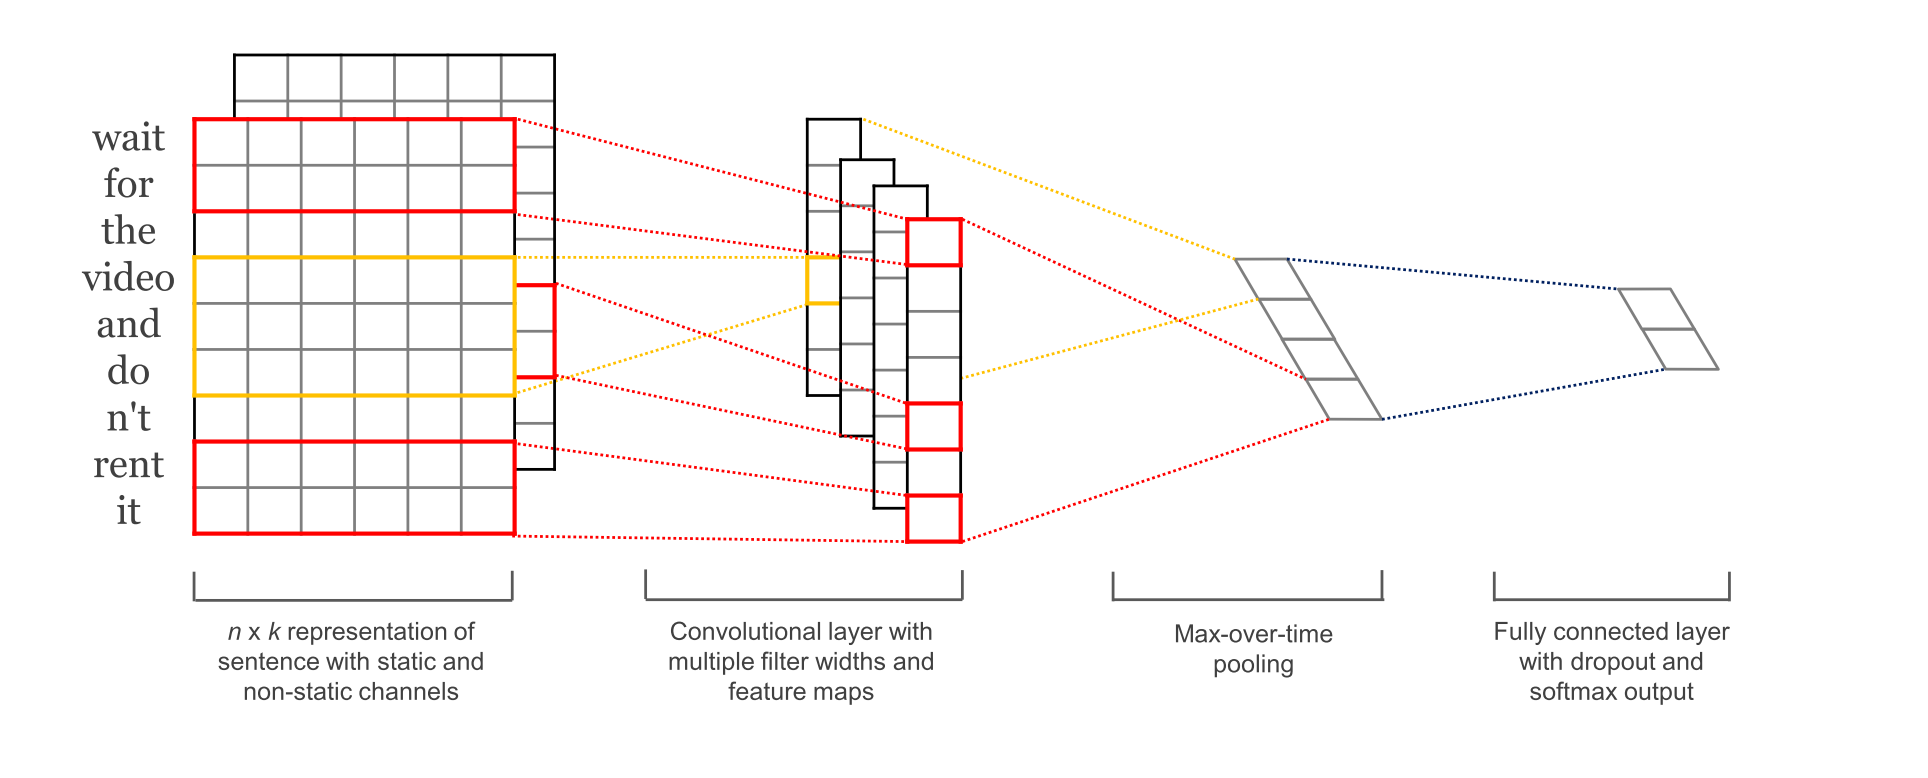
\includegraphics[width=\textwidth]{images/chapters/cnn_architecture.png}
    
    \fonte{\textcite{Kim2014}.}
\end{figure}

% Warning!! Copy/Paste
This \gls{CNN} takes into account the order of the words by stacking the corresponding embeddings for each word as they occur in the text. 
% Warning!! Copy/Paste
Then it applies multiple convolutional masks with different dimensions that correspond to the red and yellow contours in Figure~\ref{fig:cnn_model}. Mask widths are equal to word embedding size while the heights can vary. In this context, mask height can be related to the idea of N-Grams, since they embrace multiple embeddings at the same time. 
% Warning!! Copy/Paste
In the original architecture, these heights were set to three, four, and five. We added one more mask of height two, which increased classification metrics. Also, based on empirical experimentation, we set  the number of masks to ten for each of these sizes, without affecting our results, but decreasing the required training time. 

% Warning!! Copy/Paste
% Explicar sobre como esse modelo foi utilizado
In this work, we applied each of the embeddings trained in conjunction with the \gls{CNN} described to the classification of \gls{JEC} at \gls{UFSC} judgments, where Out of Vocabulary (OOV) words are replaced by an vector of random values. Thus, we trained and tested 41 models. Furthermore, due to the stochastic nature of neural networks training methods~\cite{Cohen1995}, each of these models was trained and tested 200 times and the resulting evaluation metrics were averaged. 

% Warning!! Copy/Paste
Finally, we compare the performance in classification using accuracy and macro F1-Score.


\subsection{Results and Discussion}

% Warning!! Copy/Paste
Following the steps presented in Section~\ref{sec:pipeline_representation}, we trained all 41 word embeddings representations for GloVe. 

% Warning!! Copy/Paste
To illustrate how these embeddings behave, Figure~\ref{fig:projection} shows the projection in two dimensions, using \gls{t-SNE} \cite{Maaten2008} of perplexity of 0.1, of a sample of words from \emph{general} context embedding trained with 1 billion words. Each axis corresponds to a \gls{PC}.

\begin{figure}[tb]
    \centering
    \caption{Word Embeddings projection using t-SNE}
    \label{fig:projection}
    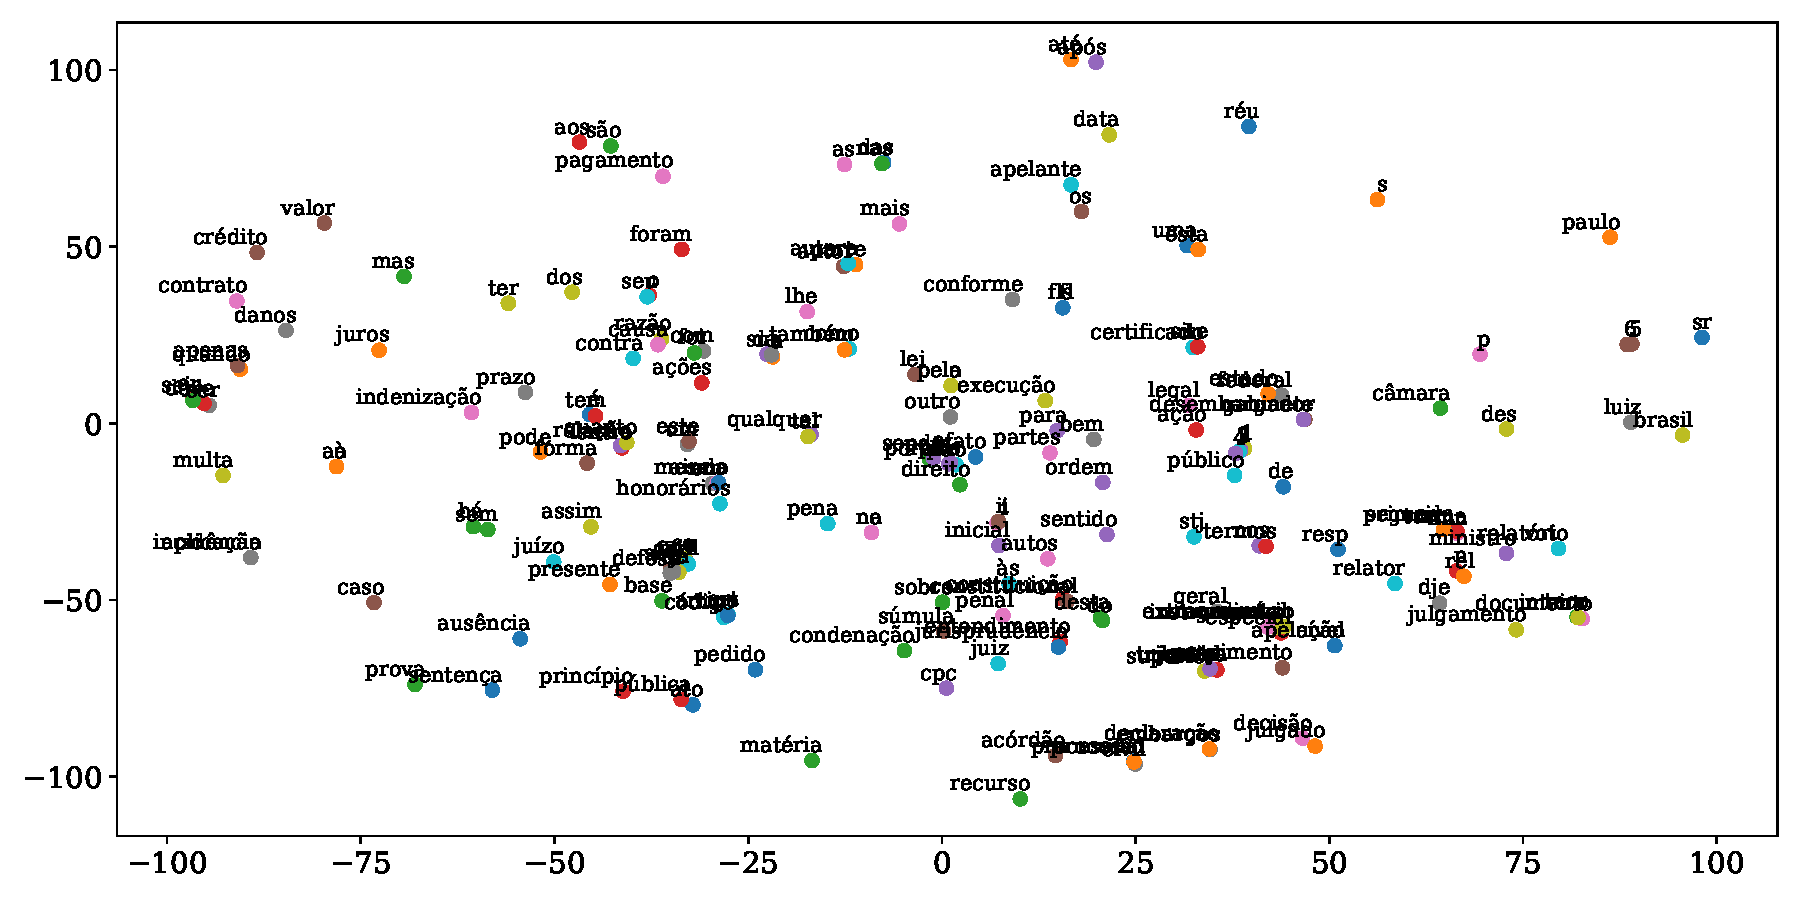
\includegraphics[width=\textwidth]{images/chapters/tsne_2000_0.1.pdf}
    
    % \fonte{\textcite{DalPont2020}.}
\end{figure}

% Warning!! Copy/Paste
%%%% FIGURE- Embeddings projection
%Using each embedding, we trained and tested  \gls{CNN} for text classification of the judgments from \gls{JEC}. %These two steps were repeated 200 times, and the evaluation metrics were averaged for each group of repetitions.

% Warning!! Copy/Paste
In Figure~\ref{fig:accuracy_plot} and \ref{fig:f1_plot}, we present the results, for accuracy and F1-Score, respectively, from test data applied to each \gls{CNN}. These results are related to pre-trained embeddings  with \emph{general}, \emph{air transport}, \emph{global} texts. 
The x-axis denotes the corpus sizes used to train the embeddings, while the y-axis represents accuracy or F1-Score. Each data point represents the average of the evaluation metric, after 200 train and test repetitions using each specific embedding. %Finally, we delimited y-axis to smaller intervals so the metrics variations could be visible.


% JH In the next section, we discuss these results.

\begin{figure}[htb]
    \centering
    \caption{Accuracy for test set from CNN in embeddings evaluation}
    \label{fig:accuracy_plot}
    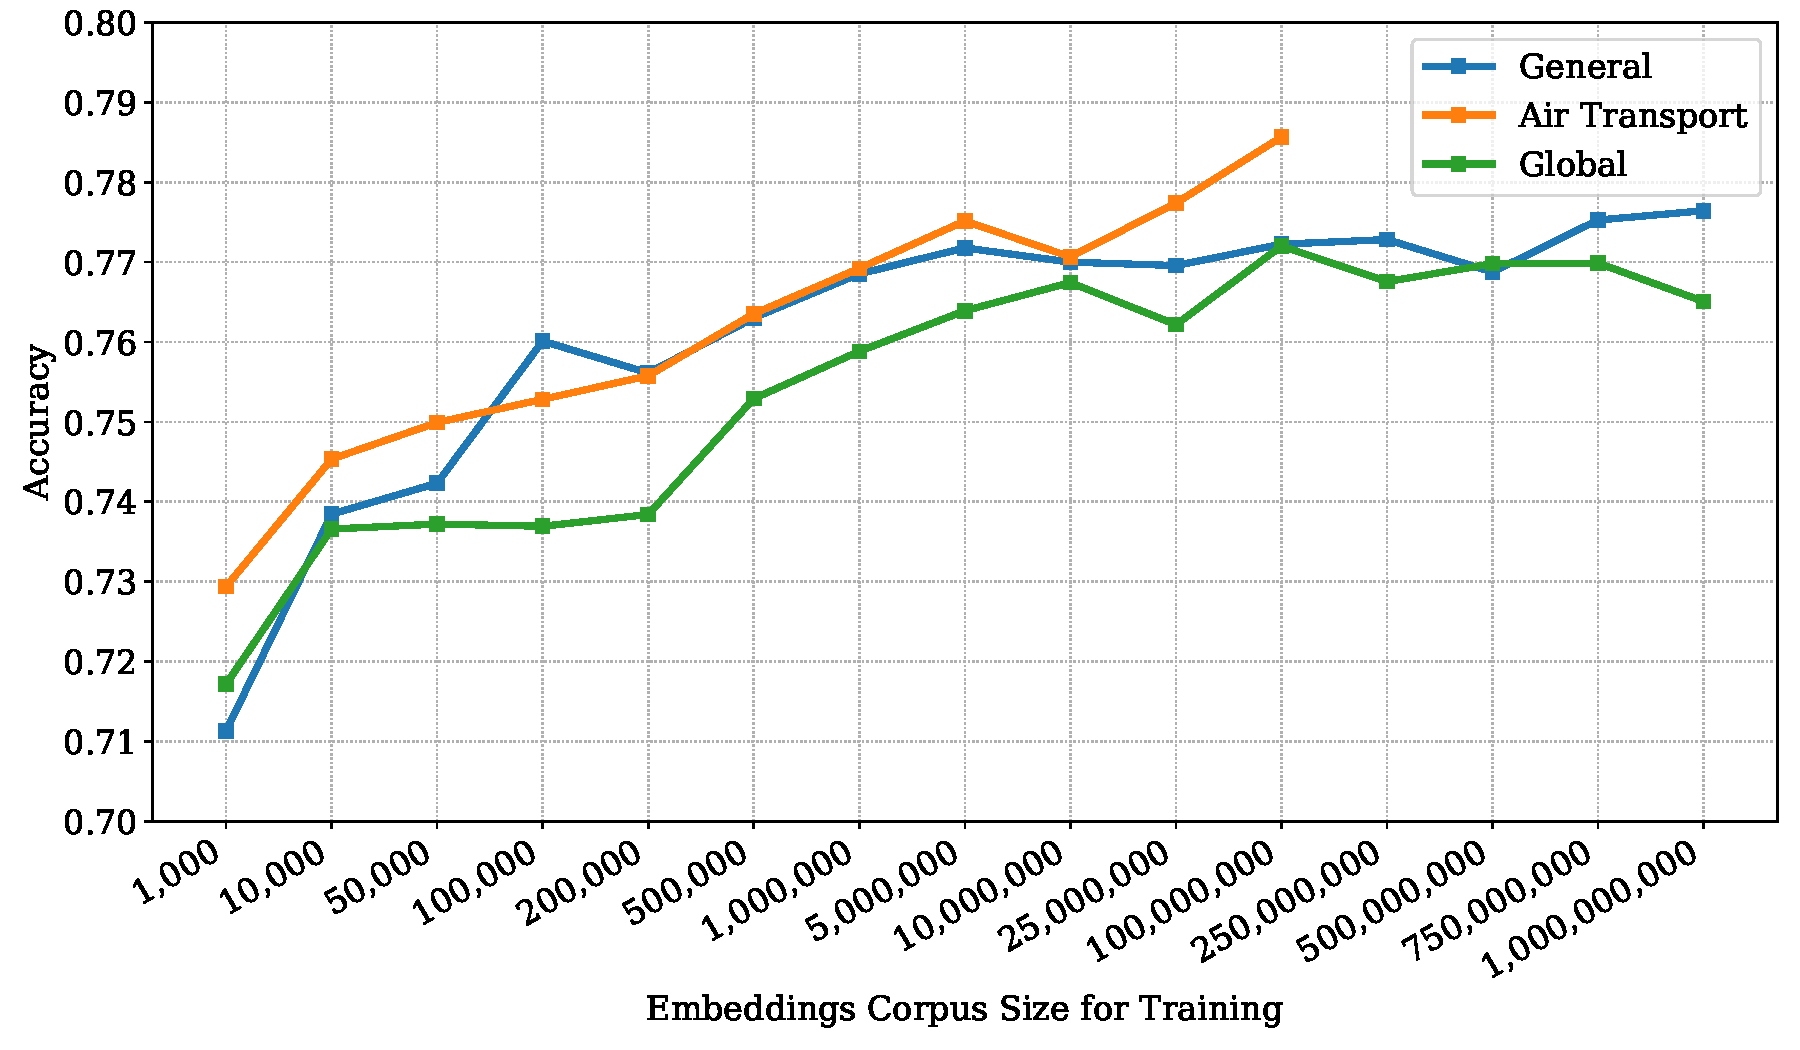
\includegraphics[width=\textwidth]{images/chapters/acc_mean_final.pdf}
    
    % \fonte{\textcite{DalPont2020}.}
\end{figure}

\begin{figure}[htb]
    \centering
    \caption{Macro F1-Score for test set from CNN  in embeddings evaluation}
    \label{fig:f1_plot}
    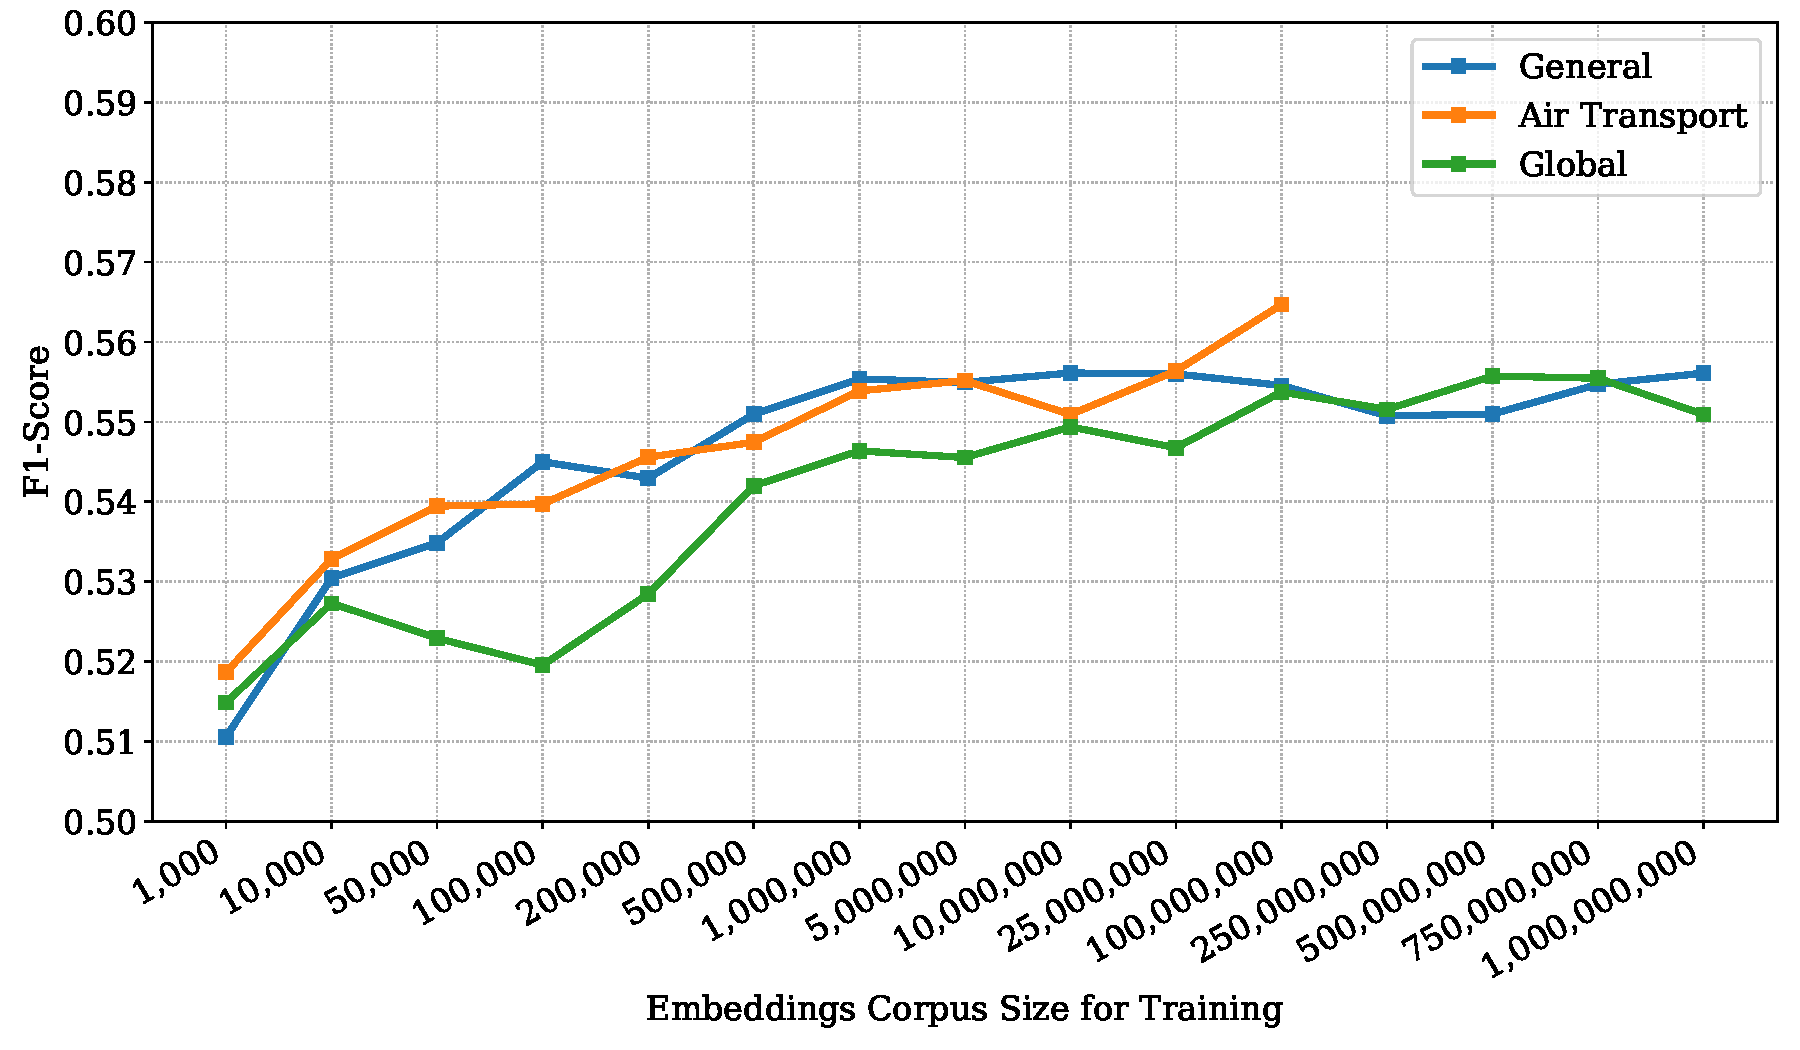
\includegraphics[width=\textwidth]{images/chapters/f1_score_mean_final.pdf}
    
    % \fonte{\textcite{DalPont2020}.}
\end{figure}

% Evaluations from context perspective
%\subsection{Discussion from Context Perspective}

% Warning!! Copy/Paste
We focus now on the part of research question regarding specificity: Does the \textit{specificity}  of the corpus used for word embeddings training impact the performance of a text classification using such representations? 

% Warning!! Copy/Paste
In terms of accuracy, when we compare \emph{global} against others (Figure~\ref{fig:accuracy_plot}), we have that higher text specificity leads to better results, for most of the corpus sizes used for embeddings training. Furthermore, when comparing \emph{general} and \emph{air transport} curves, there is a significant difference in accuracy only for the lowest and highest x-values. 
However, in terms of F1-Score, as shown in Figure~\ref{fig:f1_plot}, our observations change, once \emph{general} and \emph{air transport} curves have a similar shape. Also, for the highest corpus sizes, \emph{general} and \emph{global} curves converge to similar values of F1-Score. 
%
% Warning!! Copy/Paste
The differences in accuracy and F1-Score may emerge from the fact that our dataset to text classification is imbalanced, once the former does not take this fact into account, while the latter does. However, this result still requires further investigation. 
% Warning!! Copy/Paste
% In general, we can note that for smaller corpora sizes for embeddings training, text specificity has a more impact than for large sizes.


%\subsection{Discussion from Corpus Size Perspective}

% Warning!! Copy/Paste
Regarding the part of research question in terms of size: 
Does the \textit{size}  of the corpus used for word embeddings training impact the performance of a text classification using such representations? 

% Warning!! Copy/Paste
When we observe both accuracy and F1-Score measures from Figure~\ref{fig:accuracy_plot} and \ref{fig:f1_plot}, it is clear the tendency for improvement while increasing corpus size. However, the metrics converge with the largest corpus sizes. There are two exceptions. The first one occurs with smaller values of corpus sizes for \textit{global} curve, as it decreases in F1-Score measures. The second corresponds to the last data point in \textit{air transport} curves. The former can happen when the classifier performs poorly for some classes while gets better in others. The latter may indicate that those curves could improve if we had more significant corpus sizes related to that context.

% Warning!! Copy/Paste
In general, we can note that the greater the corpus size in embeddings training, the better are the results. However, this impact decreases as the corpus size increases until a point where more words in the corpus have little impact on the results.
